\documentclass{article}
\usepackage{microtype}
\usepackage{graphicx}
\usepackage{booktabs}
\usepackage{hyperref}
\usepackage[preprint]{icml2026}
\usepackage{amsmath,amssymb,mathtools,amsthm}
\usepackage{subcaption}
\usepackage{url}
\newtheorem{proposition}{Proposition}
\newcommand{\KernelLowNumeric}{14.3\% [12.5, 16.2]}
\newcommand{\KernelLowRank}{54.0\% [51.8, 56.2]}
\newcommand{\KernelLowJoint}{12.7\% [11.0, 14.6]}
\newcommand{\KernelLowSign}{64.3\% [62.2, 66.4]}
\newcommand{\KernelLowStrict}{3.1\% [2.5, 3.8]}
\newcommand{\KernelLowLenient}{36.6\% [33.6, 39.4]}
\newcommand{\PermLowNumeric}{55.0\% [51.8, 58.1]}
\newcommand{\PermLowRank}{80.8\% [78.7, 82.9]}
\newcommand{\PermLowJoint}{48.2\% [45.0, 51.5]}
\newcommand{\PermLowSign}{98.1\% [97.4, 98.7]}
\newcommand{\PermLowStrict}{19.5\% [17.0, 22.0]}
\newcommand{\PermLowLenient}{81.6\% [78.8, 84.2]}
\newcommand{\WrongAgreeLow}{9.3\% [7.7, 11.2]}
\newcommand{\KernelMediumNumeric}{80.8\% [77.6, 84.0]}
\newcommand{\KernelMediumRank}{90.6\% [88.7, 92.4]}
\newcommand{\KernelMediumJoint}{74.4\% [70.9, 77.7]}
\newcommand{\KernelMediumSign}{98.6\% [98.1, 99.1]}
\newcommand{\KernelMediumStrict}{51.1\% [46.7, 55.4]}
\newcommand{\KernelMediumLenient}{97.5\% [96.6, 98.3]}
\newcommand{\PermMediumNumeric}{82.0\% [79.4, 84.4]}
\newcommand{\PermMediumRank}{90.5\% [88.8, 92.2]}
\newcommand{\PermMediumJoint}{75.7\% [72.9, 78.6]}
\newcommand{\PermMediumSign}{99.8\% [99.7, 99.9]}
\newcommand{\PermMediumStrict}{54.9\% [51.7, 58.0]}
\newcommand{\PermMediumLenient}{96.9\% [95.7, 97.9]}
\newcommand{\WrongAgreeMedium}{2.5\% [1.8, 3.4]}
\newcommand{\KernelLargeNumeric}{99.8\% [99.6, 100.0]}
\newcommand{\KernelLargeRank}{97.7\% [96.7, 98.6]}
\newcommand{\KernelLargeJoint}{97.5\% [96.6, 98.4]}
\newcommand{\KernelLargeSign}{100.0\% [100.0, 100.0]}
\newcommand{\KernelLargeStrict}{94.1\% [92.3, 95.8]}
\newcommand{\KernelLargeLenient}{100.0\% [100.0, 100.0]}
\newcommand{\PermLargeNumeric}{97.3\% [96.2, 98.2]}
\newcommand{\PermLargeRank}{95.6\% [94.2, 96.8]}
\newcommand{\PermLargeJoint}{93.1\% [91.5, 94.5]}
\newcommand{\PermLargeSign}{100.0\% [100.0, 100.0]}
\newcommand{\PermLargeStrict}{83.0\% [80.4, 85.4]}
\newcommand{\PermLargeLenient}{99.9\% [99.7, 100.0]}
\newcommand{\WrongAgreeLarge}{0.7\% [0.3, 1.1]}
\newcommand{\KernelHighNumeric}{100.0\% [100.0, 100.0]}
\newcommand{\KernelHighRank}{99.4\% [98.9, 99.9]}
\newcommand{\KernelHighJoint}{99.4\% [98.9, 99.9]}
\newcommand{\KernelHighSign}{100.0\% [100.0, 100.0]}
\newcommand{\KernelHighStrict}{100.0\% [99.9, 100.0]}
\newcommand{\KernelHighLenient}{100.0\% [100.0, 100.0]}
\newcommand{\PermHighNumeric}{98.8\% [98.2, 99.3]}
\newcommand{\PermHighRank}{96.8\% [95.6, 97.9]}
\newcommand{\PermHighJoint}{95.7\% [94.4, 96.9]}
\newcommand{\PermHighSign}{100.0\% [100.0, 100.0]}
\newcommand{\PermHighStrict}{92.2\% [90.7, 93.6]}
\newcommand{\PermHighLenient}{100.0\% [100.0, 100.0]}
\newcommand{\WrongAgreeHigh}{0.2\% [0.0, 0.4]}
\newcommand{\CellMinLow}{0.3\%}
\newcommand{\CellMaxLow}{29.8\%}
\newcommand{\CertifiedLow}{0}
\newcommand{\CellMinMedium}{40.2\%}
\newcommand{\CellMaxMedium}{92.7\%}
\newcommand{\CertifiedMedium}{105}
\newcommand{\CellMinLarge}{91.4\%}
\newcommand{\CellMaxLarge}{100.0\%}
\newcommand{\CertifiedLarge}{245}
\newcommand{\CellMinHigh}{97.9\%}
\newcommand{\CellMaxHigh}{100.0\%}
\newcommand{\CertifiedHigh}{280}
\newcommand{\MainRuns}{147,456}
\newcommand{\KernelRuns}{73,728}
\newcommand{\DefaultRuns}{6,144}
\newcommand{\GameCount}{288}
\newcommand{\BackgroundGameCount}{1152}
\newcommand{\TotalCpuHours}{1.42}
\newcommand{\GamesCpuHours}{1.05}
\newcommand{\ReferenceEfficiency}{6.4e-16}
\newcommand{\TimeMin}{6.7}
\newcommand{\TimeMax}{1402.5}
\newcommand{\WarningCount}{2231}
\newcommand{\TiedCases}{0}
\newcommand{\ExhaustiveError}{1.1e-15}
\newcommand{\SolverRuns}{18,432}
\newcommand{\ExtremePackage}{277}
\newcommand{\ExtremeSvd}{0}
\newcommand{\DeficientDesigns}{3,507}
\newcommand{\DefaultLRNumeric}{0.0\% [0.0, 0.0]}
\newcommand{\DefaultLRRepeat}{91.7\% [84.4, 97.6]}
\newcommand{\DefaultHGBNumeric}{12.4\% [3.2, 23.0]}
\newcommand{\DefaultHGBRepeat}{98.5\% [96.7, 100.0]}

\icmltitlerunning{Single-run reliability of budgeted SHAP explanations}
\begin{document}
\twocolumn[
\icmltitle{When Is a Single SHAP Run Enough?\\An Exact-Reference Audit of Budgeted Tabular Explanations}
\begin{icmlauthorlist}
\icmlauthor{Autonomous Research Study}{ind}
\end{icmlauthorlist}
\icmlaffiliation{ind}{Reproducible computational study; no institutional affiliation.}
\icmlcorrespondingauthor{Autonomous research artifact}{no human correspondent}
\icmlkeywords{SHAP, reliability, interpretability, Monte Carlo approximation, tabular classification}
\vskip 0.3in
]
\printAffiliationsAndNotice{}
\begin{abstract}
A repeated explanation can be numerically accurate yet change which features are displayed as most important. We investigate when one budget-limited SHAP run reproduces a fixed prediction's exact finite-background Shapley explanation. Across German Credit, Pima Diabetes and ACS Income, three fitted classifiers per dataset, and 32 matched test cases per dataset, we enumerate every coalition of the original features and repeat the actual SHAP KernelExplainer under four coalition caps and 64 independent seeds. Numerical accuracy, top-three correctness and their intersection are evaluated separately, with 95\% case-bootstrap uncertainty. At an $8d$ interior-coalition cap, mean joint success is \KernelMediumJoint{}; at $128d$, it is \KernelHighJoint{}. The largest cap exhausts the two smaller games, while remaining an approximation on German Credit. We compare a permutation baseline and examine repeated-run agreement, averaging, default sparsification, and independent background redraws. The evidence supports a conditional answer: reliability depends on the budget, the displayed claim, the attribution gap, and the exact explanation target. Repeat agreement is a diagnostic, not a correctness certificate. The released code contains exact payoff tables, all explanation runs, and separate uncached online timings.
\end{abstract}

\section{Introduction}
A feature-attribution vector is often presented as a reason for a model's decision. For a fixed trained classifier and an unchanged applicant or patient record, users reasonably expect the displayed reasons to remain the same. Randomized approximation makes that expectation conditional on a computational budget. A plausible-looking attribution vector from a single seed gives little direct evidence about its own error. Moreover, a vector may be close to the target while choosing a different third-ranked feature, or may reproduce its own ranking while systematically suppressing contributions.

We study \emph{computational reliability}: whether a new random seed, at a specified cost, produces an explanation accurate enough for a specified use. This is narrower than establishing that a model is correct or that its explanation is causal. We hold the fitted model, explained input, probability output scale, feature grouping and empirical background fixed. This isolates approximation randomness from model retraining, alternative explanation definitions and background selection.

A useful audit needs more than agreement between approximate runs. We compute exact Shapley values for the same finite-background game by enumerating all coalitions, including the 20-feature German Credit game. This expensive audit gives a reference independent of the estimator being evaluated. It also lets us distinguish a stable wrong explanation from an unstable one, and quantify when an apparently small numerical error changes the top-three display. Online budgets remain limited: the stochastic methods receive only their allotted coalition calls, and separate direct model evaluations measure deployment latency.

Our contributions are threefold. First, we operationalize single-run reliability as a conditional seed-success probability, separately for numerical contributions, a top-three feature set, material signs and a joint criterion. We connect ranking failures to the exact cutoff gap rather than interpreting all disagreement as equally substantive. Second, we release a fully enumerated, original-feature benchmark spanning three public classification datasets and three model classes, with \KernelRuns{} Kernel SHAP runs and the same number of permutation runs. Third, controlled ablations separate finite-budget randomness from feature-selection bias and background-induced target changes. We report pointwise evidence and uncertainty rather than assert that one universal budget makes SHAP reliable.

The central empirical claims are directly testable: increasing the coalition budget raises average accuracy under this fixed-target setup; numerical and exact top-three reliability can differ substantially; and agreement between two stochastic runs does not certify correctness. These claims concern the measured configurations. They do not imply that every larger budget improves every individual seed, that every model class behaves alike, or that exact Shapley values are sufficient grounds for a consequential decision.

\section{Related work and scope}
SHAP unifies additive feature attributions and motivates Kernel SHAP's constrained weighted regression~\citep{lundberg2017}. We evaluate the maintained implementation rather than infer reliability from the axioms of exact Shapley values. Musco and Witter~\citep{musco2025} provide leverage-score sampling guarantees and improve estimation error; our question is the empirical probability that the actual library, at a limited budget, reproduces the numerical and displayed content of a fixed target. We do not propose a competing estimator or benchmark every modern sampling method.

Krishna et al.~\citep{krishna2024} study disagreement \emph{between} explanation methods and how practitioners resolve it. We instead vary the random seed of a single estimator while holding its semantic target fixed. Nogueira et al.~\citep{nogueira2018} distinguish stochastic and data-sampling effects in feature-selection stability and develop statistical measures. We use exact top-three agreement for a specific display, not a claim that it replaces their chance-corrected global stability measure. Numerical error, signs and cutoff gaps complement this strict set criterion.

Yuan et al.~\citep{yuan2023} report that resampled background datasets affect SHAP values and rankings for deep models. We treat this as variation of the game itself, and isolate it using exact values under independently drawn backgrounds. Chen et al.~\citep{chen2020} explain the distinct meanings of interventional and observational games; our conclusions are explicitly restricted to Eq.~\eqref{eq:game}. ACS Income follows the public-data construction of Ding et al.~\citep{ding2021}. The tabular benchmarking study of Gorishniy et al.~\citep{gorishniy2021} motivates using multiple model types rather than treating one architecture as representative. We use modest CPU baselines, not an architecture competition. The contribution is the joint, exact-reference audit and its reproducible evidence, not a claim of being the first study of SHAP variability.

\section{A conditional reliability question}
\label{sec:method}
Let $f:\mathcal X\to[0,1]$ be a \emph{fixed fitted} positive-class probability model, $x$ a fixed test input, and $Z=(z_1,\ldots,z_B)$ a fixed training-background sample. The players are the $d$ original variables, including whole categorical variables rather than individual dummy columns. We study the finite interventional game
\begin{equation}
 v_{x,Z}(S)=\frac1B\sum_{b=1}^B f(x_S,z_{b,\bar S}),\quad S\subseteq[d].
 \label{eq:game}
\end{equation}
All absent variables come from the \emph{same} background row. This preserves their joint distribution with each other, but breaks their dependence with present variables. We do not estimate observational conditional expectations, use survey weights, or interpret interventions causally. The exact target is
\begin{equation}
 \phi_j=\sum_{S\subseteq[d]\setminus\{j\}}
 \frac{v(S\cup\{j\})-v(S)}{d\binom{d-1}{|S|}}.
 \label{eq:shap}
\end{equation}
For a stochastic algorithm $A$ with budget $m$ and seed $U$, $\widehat\phi=A(v,m,U)$. Our question is a probability over $U$, conditional on $f,x,Z$. Training-seed uncertainty, background uncertainty, numerical approximation, and causal validity are different questions. We separately vary $Z$ in a secondary experiment.

\subsection{What counts as a reliable explanation?}
\label{sec:metrics}
Let $T_3(a)$ select the three largest absolute coordinates of $a$, breaking ties by original variable order. Define
\begin{align}
 E&=\|\widehat\phi-\phi\|_\infty,\\
 N_\epsilon&=\mathbf1\{E\leq\epsilon\},\quad
 K=\mathbf1\{T_3(\widehat\phi)=T_3(\phi)\},\\
 J_\epsilon&=N_\epsilon K,\qquad
 p_J(x;m)=\Pr_U(J_\epsilon=1).
\end{align}
Our primary tolerance is $\epsilon=.01$: every feature contribution must be within one percentage point of predicted probability. This is a transparent engineering tolerance, not a medically or legally validated standard. We repeat the numerical analysis at $.005$ and $.02$. A top-three display has a separate, stricter requirement: exactly the same set. This can penalize negligible differences near ties; we report the cutoff gap to expose this sensitivity. We also measure correct signs for \emph{all} features with $|\phi_j|\geq .01$, and relative $\ell_1$ error $\|\widehat\phi-\phi\|_1/\max(\|\phi\|_1,10^{-12})$.

We call an instance computationally reliable at a chosen budget and criterion when its seed-success probability is at least $.95$. This is a definition to evaluate, not an assumption. A mean over instances cannot establish it for every instance. We report mean success and a conservative per-instance check: the one-sided $95\%$ Clopper--Pearson lower bound for $p_J$ must exceed $.95$. With $64$ successes out of $64$, that bound is $.05^{1/64}>.95$; with a failure, it does not pass. These are pointwise checks with no familywise adjustment, and the resulting counts are descriptive rather than simultaneous guarantees.

\subsection{Agreement is observable; correctness needs a target}
For two independent runs, repeat top-three agreement is
\begin{equation}
 R=\mathbf1\{T_3(\widehat\phi^{(1)})=T_3(\widehat\phi^{(2)})\}.
\end{equation}
If $q_A=\Pr\{T_3(\widehat\phi)=A\}$, then $\Pr(R=1)=\sum_Aq_A^2$, while top-three correctness is $q_{T_3(\phi)}$. Agreement alone cannot identify which set is correct. We therefore measure $\Pr(K^{(1)}=0\mid R=1)$ as an empirical false-reassurance diagnostic. The analogous joint agreement requires $R=1$ and $\|\widehat\phi^{(1)}-\widehat\phi^{(2)}\|_\infty\leq .01$. We use disjoint seed pairs to avoid treating the quadratically many overlapping pairs as independent evidence.

The margin explains one source of the discrepancy. Write $|\phi|_{(j)}$ for the $j$th largest absolute attribution and $\Delta_3=|\phi|_{(3)}-|\phi|_{(4)}$. The elementary implication
\begin{equation}
 E<\Delta_3/2\ \Longrightarrow\ K=1
 \label{eq:margin}
\end{equation}
holds because absolute values change by at most $E$. Similarly, $E<|\phi_j|$ preserves a nonzero feature's sign. Thus small numerical error need not preserve a ranking with a small cutoff gap. These are deterministic sensitivity statements, not new statistical guarantees; Appendix~\ref{app:proof} gives the proof. Exact gaps are available in an audit, but ordinarily unavailable in deployment.

\subsection{Estimators and an honest budget}
\label{sec:budget}
The primary method is the actual \texttt{shap.KernelExplainer} in SHAP~0.51.0, with identity link and \texttt{l1\_reg=0}. This evaluates the library's size-stratified, complement-paired coalition sampling and constrained weighted regression, including its singular-design fallback. We disable feature selection to target the full vector in Eq.~\eqref{eq:shap}; a separate ablation restores the package's default \texttt{num\_features(10)}. We remove only columns equal to $x$ in \emph{every} background row, matching the library's varying-feature shortcut, and restore their zero coordinates afterward. Other model-dummy features remain in the game.

The requested interior-coalition cap is
\begin{equation}
 m=\min\{c d,2^d-2\},\quad c\in\{2,8,32,128\}.
\end{equation}
The implementation may spend less, particularly when fewer than $d$ columns vary. We save actual counts. Exhaustion is capped at $2^{d_a}-2$ for $d_a$ active columns. For a fresh real-data KernelExplainer, an interior payoff costs $B$ model rows; initialization uses $B$ rows for $v(\varnothing)$ and one row for $f(x)$. Thus actual raw model rows are $B(m_{\rm spent}+1)+1$ in this setting. Coalitions are a portable budget axis, but not a universal time unit.

The comparison estimator averages feature marginal contributions along uniformly sampled permutations, pairing each order with its reversal. A pair spends $2(d_a-1)$ interior payoffs. We use $\lfloor\min(m,2^{d_a}-2)/[2(d_a-1)]\rfloor$ pairs; repeated coalitions remain charged, and leftover budget is unused. The methods therefore share a budget \emph{cap}, not identical evaluation counts. Kernel SHAP deduplicates its sampled masks and can enumerate a small game exactly; this baseline does not. Full enumeration is an additional deterministic accuracy control, not a deployment baseline at a smaller cost.

\subsection{Exact offline audit and uncertainty}
Every main reference enumerates \emph{all} $2^d$ payoffs of Eq.~\eqref{eq:game}, using double precision, and applies Eq.~\eqref{eq:shap}. There is no high-budget Monte Carlo proxy for truth. We cache these payoffs, expose the exact game as a binary-mask model to KernelExplainer, and replicate its randomness cheaply. This preserves sampled payoffs and regression, but its lookup time is \emph{not} deployment time. A direct raw-model comparison and independent permutation-sum checks validate the wrapper (Appendix~\ref{app:validation}). Separate uncached runs measure online time.

For each dataset we sample $32$ held-out cases, use the same cases across the three fitted models, and run $64$ independent explanation seeds at each budget. A cell's success rate first averages seeds within each case, then averages cases. We obtain $95\%$ percentile intervals with $2{,}000$ bootstrap resamples of cases. For model-averaged or overall summaries, the bootstrap preserves matched cases across models and resamples within each dataset; datasets receive equal weight. The models and datasets themselves are fixed, not random draws from a model or dataset population. Intervals quantify test-case heterogeneity under this design; they do not quantify training-split variation or establish a universal reliability threshold. We do not treat seeds, matched models, or overlapping background pairs as independent test cases, and make no multiple-testing significance claims.

\section{Experimental design and results}
\label{sec:experiments}
\subsection{Public tables and fixed classifiers}
We use both main datasets requested for the study, German Credit and ACS Income, plus Pima Diabetes to obtain a lower-dimensional exact control. German has 20 original features; Pima has 8; ACS Income has 10. We use California 2018 ACS person records through folktables' standard task definition~\citep{ding2021}, not the Adult benchmark. The different dimensions make explicit when a budget reaches complete enumeration. They are not a controlled experiment isolating dimension from dataset content.

Each dataset has a stratified 75/25 training/test split. ACS training is capped at 20,000; the test pool is retained. We train logistic regression (LR), random forest (RF), and histogram gradient boosting (HGB) with fixed hyperparameters and seed. Logistic regression uses training-standardized numeric features and one-hot categorical variables; trees use original numeric/category codes. The games always use original features as players. Imputation is learned on training data. Table~\ref{tab:data} gives exact sample counts and predictive scores, which contextualize the fitted models but are not explanation-quality measures. Appendix~\ref{app:setup} specifies preprocessing and hyperparameters.

\begin{table*}[t]
\centering\small
\begin{tabular}{lrrrrrr}
\toprule
Dataset & $n$ & Train & Test & $d$ & LR/RF/HGB AUC & LR/RF/HGB acc. \\
\midrule
German & 1,000 & 750 & 250 & 20 & 0.762/0.780/0.788 & 0.728/0.708/0.720 \\
Pima & 768 & 576 & 192 & 8 & 0.821/0.824/0.796 & 0.781/0.755/0.750 \\
ACS & 195,665 & 20,000 & 48,917 & 10 & 0.892/0.883/0.897 & 0.814/0.805/0.817 \\
\bottomrule
\end{tabular}
\caption{Datasets after task filtering, training/test sizes and fixed-model predictive performance. LR/RF/HGB entries follow that order. ACS is unweighted California 2018 ACSIncome; its capped training sample does not change the test size.}
\label{tab:data}
\end{table*}

The main background is a fixed uniform sample of 16 training records, shared across cases and models within a dataset. This small background keeps online explanation costs realistic and makes the target completely explicit; it is not asserted to represent the population adequately. Each dataset contributes 32 uniformly selected test cases, matched across fitted models. There are \GameCount{} exact main games, \MainRuns{} stochastic main explanations across two estimators, and \DefaultRuns{} extra default-regularized Kernel explanations. Independent background redraws produce another \BackgroundGameCount{} exact games on eight cases per smaller dataset.

\subsection{Numerical accuracy and displayed-feature accuracy}
\label{sec:primary}
Table~\ref{tab:main} reports joint success, the fraction of runs satisfying both $E\leq .01$ and exact top-three equality. Every interval bootstraps the 32 cases in its cell. Figure~\ref{fig:accuracy} separates the two requirements. Over the nine equally weighted fitted-model cells, Kernel SHAP's joint success is \KernelLowJoint{} at $2d$, \KernelMediumJoint{} at $8d$, \KernelLargeJoint{} at $32d$, and \KernelHighJoint{} at $128d$. These averages describe this benchmark and are not a probability of reliability on an arbitrary future dataset.

At $8d$, numerical success is \KernelMediumNumeric{}, while top-three success is \KernelMediumRank{}. The criteria answer different questions: numerical tolerance controls all coordinates in probability units; a top-three display asks a discrete membership question. Relaxing the numerical tolerance to $.02$ yields \KernelMediumLenient{} numerical success, and tightening it to $.005$ yields \KernelMediumStrict{}. A threshold must therefore accompany any claim that an explanation is accurate enough. Material-sign success at this budget is \KernelMediumSign{}; including tiny near-zero features in a sign metric would ask a substantially more sensitive question.

\begin{table*}[t]
\centering\small
\begin{tabular}{llrrrr}
\toprule
Data & Model & $2d$ & $8d$ & $32d$ & $128d$ \\
\midrule
German & LR & 9.8 [6.3, 13.4] & 90.7 [84.5, 95.9] & 96.6 [92.9, 99.5] & 97.9 [94.4, 100.0] \\
German & RF & 20.3 [15.3, 25.5] & 91.3 [85.7, 96.2] & 96.2 [92.4, 99.2] & 98.4 [96.0, 99.9] \\
German & HGB & 0.3 [0.0, 0.8] & 48.6 [37.6, 59.1] & 95.8 [91.6, 98.8] & 98.6 [95.9, 100.0] \\
Pima & LR & 29.8 [22.1, 38.2] & 88.8 [81.3, 95.1] & 100.0 [100.0, 100.0] & 100.0 [100.0, 100.0] \\
Pima & RF & 23.5 [18.2, 29.1] & 92.7 [87.4, 96.9] & 100.0 [100.0, 100.0] & 100.0 [100.0, 100.0] \\
Pima & HGB & 1.1 [0.5, 1.7] & 40.2 [30.4, 50.5] & 100.0 [100.0, 100.0] & 100.0 [100.0, 100.0] \\
ACS & LR & 11.2 [6.9, 15.8] & 74.2 [64.8, 83.1] & 98.3 [95.5, 100.0] & 100.0 [100.0, 100.0] \\
ACS & RF & 16.5 [12.1, 21.0] & 91.1 [85.9, 95.2] & 99.5 [98.9, 100.0] & 100.0 [100.0, 100.0] \\
ACS & HGB & 2.2 [1.1, 3.4] & 52.1 [39.5, 64.7] & 91.4 [86.1, 95.6] & 100.0 [100.0, 100.0] \\
\bottomrule
\end{tabular}
\caption{Unregularized Kernel SHAP joint success: numerical maximum error at most $.01$ \emph{and} exact top-three set. Percent, with 95\% case-bootstrap intervals. Caps refer to interior coalitions and are further capped at complete enumeration of active columns. Each cell uses 32 cases and 64 seeds per case.}
\label{tab:main}
\end{table*}

\begin{figure*}[t]
\centering
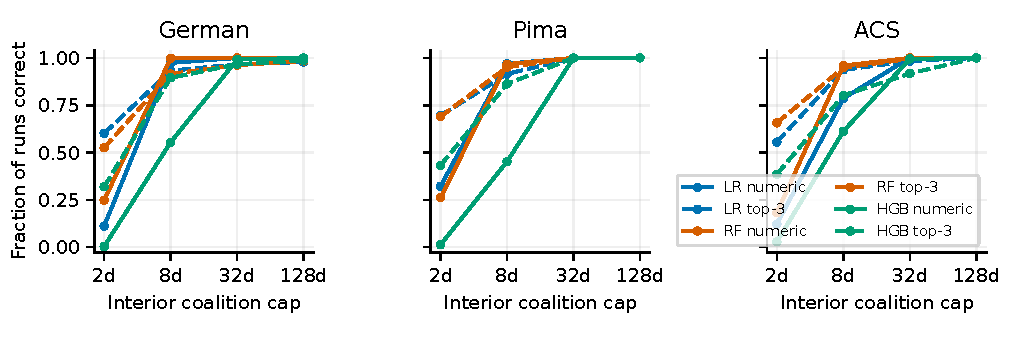
\includegraphics[width=\textwidth]{figures/accuracy.pdf}
\caption{Numerical success (solid) and exact top-three correctness (dashed), for the actual unregularized KernelExplainer. Lines are case-averaged descriptive means; joint-rate intervals appear in Table~\ref{tab:main}. Complete enumeration occurs by $32d$ for Pima and by $128d$ for ACS. The $128d$ German cap still samples only a small fraction of its coalition space.}
\label{fig:accuracy}
\end{figure*}

The smaller games reach an instructive positive control: Pima has only $2^8-2$ interior coalitions and ACS $2^{10}-2$. Their largest caps enumerate the whole active game, eliminating sampling randomness rather than merely reducing it. German's $128d$ cap remains approximate. Thus the high-budget overall mean should not be read as evidence that a fixed polynomial budget always suffices in higher dimensions. The nine cell means at $8d$ range from \CellMinMedium{} to \CellMaxMedium{}; the corresponding high-budget range is \CellMinHigh{} to \CellMaxHigh{}.

Averaging over inputs also hides difficult inputs. Pointwise lower-bound checks support $p_J\geq .95$ for \CertifiedMedium{} of 288 model/case pairs at $8d$ and \CertifiedHigh{} at $128d$. These checks require all 64 observed seeds to succeed; failing the check is inconclusive, not proof that $p_J<.95$. Passing cases at the exhaustive caps are deterministic controls for the chosen game. Neither their counts nor the bootstrap intervals certify every test input.

\subsection{Budget-matched permutation comparison}
\label{sec:baseline}
Figure~\ref{fig:baseline} compares joint success under the same interior-payoff caps. The reversal-paired permutation estimator is substantially stronger than low-budget Kernel SHAP in this experiment: its overall $2d$ joint success is \PermLowJoint{}, versus \KernelLowJoint{} for Kernel. At $8d$, it achieves \PermMediumJoint{}, and at $128d$, \PermHighJoint{}. This comparison neither establishes a universal winner nor implies that the same number of unique coalitions is spent: Kernel deduplicates while permutation paths can revisit a coalition and leave a remainder of the cap unused.

The lowest Kernel budget is close to the regression design's degrees of freedom, especially with complement pairing. The package emitted \WarningCount{} warnings in the main repetitions, retained together with all outputs; its singular-matrix fallback is not excluded. A warning-free run is also not a correctness certificate. At the largest smaller-game cap, Kernel's exact enumeration is a structural advantage over the random permutation baseline. The comparison identifies an interaction of budget and implementation, rather than a statement about the exact Shapley solution itself. A post hoc solver audit replays all \SolverRuns{} lowest-budget designs exactly: \ExtremePackage{} package outputs have $E>1$, versus \ExtremeSvd{} after replacing the normal-equation solve with SVD least squares. However, SVD only slightly improves low-budget success (Appendix~\ref{app:solver}); inadequate sampling remains a problem after extreme numerical failures are removed.

\begin{figure*}[t]
\centering
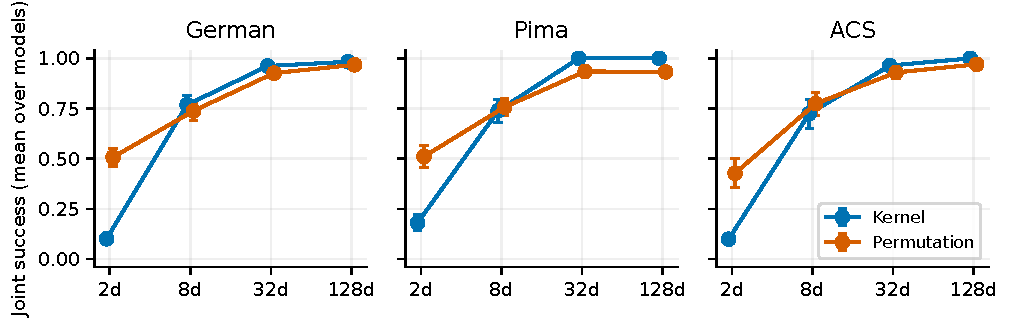
\includegraphics[width=\textwidth]{figures/baseline.pdf}
\caption{Joint success for Kernel SHAP and reversal-paired uniform permutation sampling under matched budget caps. Means average equally over the three fixed models. Error bars are 95\% bootstraps of matched cases within each dataset. Full enumeration benefits Kernel on the two smaller games; the permutation baseline continues random path sampling.}
\label{fig:baseline}
\end{figure*}

\subsection{Near ties and repeat agreement}
\label{sec:ties}
Figure~\ref{fig:margin} stratifies the $8d$ Kernel results by the exact third-versus-fourth absolute-attribution gap. The numerical and ranking criteria separate most clearly in the small-gap stratum. This descriptive analysis is consistent with Eq.~\eqref{eq:margin}; it does not identify the gap as the sole cause of error, because gap, model and data difficulty co-vary. There are \TiedCases{} exact or numerically negligible ($<10^{-12}$) cutoff ties among the 288 main model/case games. A deterministic tie rule makes the metric reproducible, not substantively important.

Two runs can choose the same incorrect set. Pooling disjoint seed pairs with equal dataset/model weights, the estimated fraction of agreeing top-three pairs that agree on a wrong set is \WrongAgreeLow{} at $2d$, \WrongAgreeMedium{} at $8d$, and \WrongAgreeHigh{} at $128d$. These are conditional descriptive rates with matched-case bootstrap uncertainty; they are not predictions for a deployment that selects its own examples or thresholds. Their purpose is to show why observing agreement and measuring target correctness are different operations. The released per-case analysis also measures agreement requiring numerical closeness.

\begin{figure}[t]
\centering
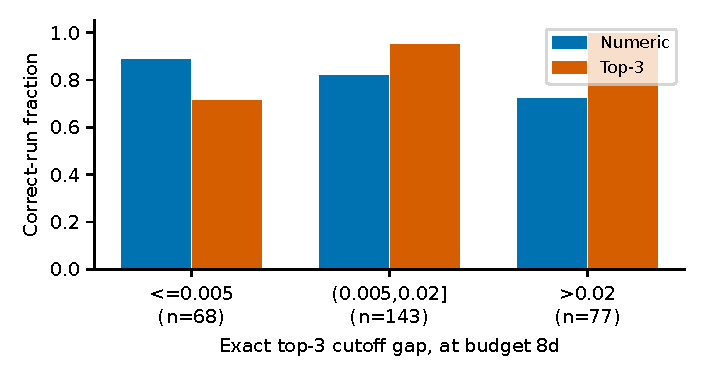
\includegraphics[width=\columnwidth]{figures/margin.pdf}
\caption{Descriptive $8d$ Kernel accuracy by exact top-three cutoff gap. Counts are model/case games, with the same test cases reused across models; bars are not independent-population estimates. Close rankings can change even when the numerical tolerance is met.}
\label{fig:margin}
\end{figure}

\subsection{Settings that change the answer}
\label{sec:ablations}
\paragraph{Default feature selection.}
Table~\ref{tab:reg} compares unregularized Kernel SHAP with its default top-10 feature selection on German Credit at $128d$, using the same coalition seeds. A sparse output is not the unrestricted target of Eq.~\eqref{eq:shap}. Consequently, increased repeatability does not automatically mean improved full-vector accuracy. For HGB, default repeat top-three agreement is \DefaultHGBRepeat{}, but numerical success is only \DefaultHGBNumeric{}. For LR, numerical success is \DefaultLRNumeric{}. The ablation reports both numerical and top-three accuracy alongside repeat top-three agreement; it should not be described as isolated Monte Carlo noise. All 20 original players remain in the reference even when the estimator selects only ten.

\begin{table*}[t]
\centering\small
\begin{tabular}{llrrr}
\toprule
Model & Regularization & Numeric & Top-3 & Repeat top-3 \\
\midrule
LR & None & 100.0 [100.0, 100.0] & 97.9 [94.4, 100.0] & 97.1 [92.8, 100.0] \\
LR & Top 10 & 0.0 [0.0, 0.0] & 78.3 [63.7, 90.6] & 91.7 [84.4, 97.6] \\
RF & None & 100.0 [100.0, 100.0] & 98.4 [96.0, 99.9] & 97.5 [94.2, 99.8] \\
RF & Top 10 & 92.4 [83.7, 99.3] & 93.7 [85.6, 99.1] & 95.3 [90.9, 98.9] \\
HGB & None & 100.0 [100.0, 100.0] & 98.6 [95.9, 100.0] & 98.4 [95.3, 100.0] \\
HGB & Top 10 & 12.4 [3.2, 23.0] & 93.6 [84.1, 100.0] & 98.5 [96.7, 100.0] \\
\bottomrule
\end{tabular}
\caption{German, $128d$: numerical correctness, top-three correctness and repeat top-three agreement. Percent with 95\% case-bootstrap intervals. ``Top 10'' is the actual SHAP 0.51.0 default, not an assumed default for other versions. Coalition seeds are paired with the unregularized condition.}
\label{tab:reg}
\end{table*}

\paragraph{Background redraws change the target.}
For Pima and ACS, we use eight selected inputs, all models, and eight independent training-background draws at each of $B=4,16,64$. We compute exact Shapley values under each draw, so disagreement here cannot be blamed on the attribution estimator. Table~\ref{tab:bg} compares all 28 pairs of backgrounds within each case, keeping those dependent pairs inside a case for inference. Increasing $B$ improves numerical agreement, but need not make a strict top-three display identical. These are comparisons between finite-sample targets, not errors relative to a known population-background Shapley value. The smaller sample of eight cases warrants cautious interpretation of its intervals.

\begin{table*}[t]
\centering\small
\begin{tabular}{llrrr}
\toprule
Dataset & $B$ & Top-3 agreement & $\|\Delta\phi\|_\infty\leq .01$ & Mean $\|\Delta\phi\|_\infty$ \\
\midrule
Pima & 4 & 34.7 [25.1, 44.2] & 0.0 [0.0, 0.0] & 0.104 [0.085, 0.125] \\
Pima & 16 & 54.6 [43.2, 66.5] & 0.3 [0.0, 0.7] & 0.067 [0.057, 0.077] \\
Pima & 64 & 82.3 [69.9, 93.8] & 7.3 [4.8, 10.4] & 0.027 [0.024, 0.031] \\
ACS & 4 & 17.3 [11.0, 24.3] & 0.0 [0.0, 0.0] & 0.132 [0.121, 0.144] \\
ACS & 16 & 30.7 [24.6, 37.6] & 0.0 [0.0, 0.0] & 0.064 [0.057, 0.072] \\
ACS & 64 & 56.1 [46.6, 66.2] & 2.8 [1.5, 4.2] & 0.030 [0.028, 0.032] \\
\bottomrule
\end{tabular}
\caption{Agreement of \emph{exact} explanations across independent background draws. Model means receive equal weight; intervals bootstrap the eight matched cases in each dataset, conditional on the eight saved draws per case/size. Top-three and numerical-agreement entries are percentages; maximum-error differences are in probability units.}
\label{tab:bg}
\end{table*}

\paragraph{Averaging and real cost.}
Four-run averaging of the lowest-budget package estimates is markedly worse than a single $8d$ run in all three datasets (Appendix~\ref{app:averaging}). This is a result for this low-budget implementation, partly affected by extreme numerical outputs; it is not a general argument against independent averaging. The comparison reports endpoint and saturation caveats rather than assuming perfect cost equality. Appendix~\ref{app:timing} reports direct, uncached online timings. Across the measured cells, median Kernel latency ranges from \TimeMin{} to \TimeMax{} milliseconds on the constrained CPU host. These use one input per cell and include contention; a production latency budget should be profiled on its own hardware and input distribution.

\section{Discussion and limitations}
\label{sec:discussion}
The evidence supports \emph{conditional} reliability. A single run can be sufficient for a specified finite-background explanation at a specified tolerance and budget, especially when the game is fully enumerated or its important features are well separated. It is not defensible to infer that status from one visually plausible plot, a predictive AUC, or an unspecified claim of ``stable SHAP.'' Numerical contributions, feature-set membership, and signs should be audited as distinct claims. An exact additive accounting identity is useful for validation but does not ensure individual coordinates are accurate.

For a deployment audit, first fix the output scale, feature grouping, background and tolerance. Then profile the real model's time per explanation, repeat seeds on held-out cases, and compare against exact values where feasible or an independently validated reference with quantified uncertainty. Report difficult inputs, not just the average. If the intended decision only uses a top-three display, examine its cutoff separation and consider showing a near-tie group instead of implying an exact ordering. If individual contributions matter, require a numerical error criterion as well. The deterministic margin statement helps interpret an audit; it does not turn a gap measured from one approximate vector into a guaranteed error bound.

Repeated agreement is useful for detecting some failures but cannot certify accuracy by itself. Default sparse regression can change which vector is estimated, and an exact explanation under one small background can differ from another equally exact explanation under a redraw. Fixing a seed merely makes an output reproducible. It does not establish that another seed would reproduce it or that it matches the chosen target. Similarly, averaging several cheap runs is a budget policy whose benefits must be measured, including duplicate evaluations and initialization.

The study has material limits. We examine three datasets, three modest fitted models and 32 test inputs per dataset, with one split and training seed. This isolates the question asked but does not measure model-retraining uncertainty or generalize statistically over datasets. German's original variables are substantially more numerous than those of the other tables, but dimension is confounded with task and feature distributions. Tree category codes impose an ordering, and logistic probability-scale explanations are nonlinear even though the underlying logit is additive. We do not evaluate neural tabular models, conditional SHAP, every library default, leverage sampling, exact TreeSHAP, alternative probability calibration, or all display sizes. Deterministic specialized algorithms could remove sampling variability while retaining other sources of explanation uncertainty.

Our backgrounds are deliberately small finite samples, and the exact reference is exact \emph{only for that empirical game}. It does not recover a population conditional expectation, prevent implausible masked combinations, or establish a scientifically appropriate attribution target. Background-sensitivity intervals use only eight cases and condition on saved draws. Case-bootstrap intervals do not include uncertainty from another train/test split, another model seed or unsampled rare inputs. Pointwise lower-bound checks have no simultaneous coverage guarantee. The chosen one-percentage-point tolerance and exact top-three set are explicit conventions, not validated measures of human utility or harm. Near-tie exchanges can be numerically harmless even when our strict display criterion fails.

Finally, offline enumeration is feasible here because there are at most 20 original players. It is exponential and unsuitable as the online policy for a large-feature production model. The cached audit cannot by itself predict production latency; our separate online measurements are limited to five trials of one input per cell on a shared CPU quota. These boundaries are part of the result: a reliability claim must name its target, cost, metric and uncertainty before it can be transferred to a new setting.

\section{Conclusion}
Under an explicitly fixed interventional game, a single SHAP run has a measurable probability of reproducing the exact explanation, and that probability varies with its computational budget and the claim extracted from the vector. The exact-reference audit shows why numerical tolerance, top-feature agreement and background choice must be assessed separately. A conditional, budgeted reliability statement is supported; an unconditional endorsement of one stochastic explanation is not.


\section*{Impact Statement}
This work evaluates numerical reproducibility of explanations of fixed classifiers. A reliable approximation to a chosen Shapley game does not validate a credit or health decision, establish fairness, or make feature effects causal. The historical datasets contain protected attributes and limited populations; they are used for a computational audit rather than deployment. We report neither individual records nor recommendations about real people. Reporting uncertainty and near-tie sensitivity may reduce overconfidence in single explanations, but no automated acceptance rule developed here should replace domain-specific review. Data access uses public sources; source licenses and Census terms are documented in the accompanying repository.

\bibliography{references}
\bibliographystyle{icml2026}
\clearpage
\appendix
\section{Data, models and reproducibility details}
\label{app:setup}
All experiments use public binary classification tables. German Credit uses the UCI mixed-type 20-variable version, with original label 2 (bad credit) as positive. Pima uses OpenML id 37, version 1; zero glucose, blood pressure, skinfold thickness, insulin and BMI are treated as missing, with training-median imputation. We neither deduplicate nor remove rows. ACS uses folktables 0.0.12, \texttt{ACSIncome}, California, 2018, 1-Year person records. The package's standard filters require age greater than 16, personal income greater than 100, positive weekly working hours, and person weight at least one; the target is personal income above \$50,000. The ten features are age, class of worker, education, marital status, occupation, birthplace, relationship, usual weekly hours, sex and race. We use the source's numeric category codes for trees, with no population weighting. This is an unweighted record-level computational benchmark, not an ACS population estimate.

The master seed is 20261102. A stratified 75/25 split defines training and test pools. For ACS only, stratified subsampling limits training to 20,000 observations. Median imputation is fitted on training records; logistic numerical variables are standardized and categorical variables one-hot encoded with unknown categories ignored. The entire encoded group is replaced together when masking an original categorical variable. For trees, each original feature occupies one column and category codes have a numerical ordering; this modeling choice is held fixed throughout. It need not be the best categorical-data modeling choice.

The logistic model uses $C=1$ and at most 2,000 solver iterations. Random forest uses 64 trees, maximum depth 6 and minimum leaf size 5. Histogram gradient boosting uses 80 iterations, at most 15 leaves per tree and $\ell_2$ regularization 1. Remaining scikit-learn defaults are pinned by the environment. We do no tuning or feature selection during training. Each cell has one training seed, as the experiment conditions on the resulting model. A dataset-specific RNG selects 32 test cases and 16 training-background rows without replacement; the selections are matched across models. Full original row indices, fitted preprocessing and models are saved in \texttt{data/*.joblib}.

Explanation seeds are generated by \texttt{numpy.random.SeedSequence} from the master seed and dataset, model, case, budget, replicate and method identifiers. Kernel and permutation seeds use distinct method identifiers. Kernel's unregularized and top-10 ablations reuse the same coalition seeds to reduce unnecessary sampling differences. Separate seeds control the background draws, online timing trials and bootstrap. The implementation stores the actual active columns, coalition counts, all warnings, every estimate, and all exact references.

\section{Why the margin implication holds}
\label{app:proof}
For any coordinate, $\big||\widehat\phi_j|-|\phi_j|\big|\leq E$. If $j\in T_3(\phi)$ and $k\notin T_3(\phi)$ with $\Delta_3>0$, then
\begin{align*}
 |\widehat\phi_j|-|\widehat\phi_k|
 &\geq |\phi_j|-|\phi_k|-2E\\
 &\geq \Delta_3-2E.
\end{align*}
This is positive when $E<\Delta_3/2$, so no outside coordinate can enter the top-three set. If $\Delta_3=0$, the strict sufficient condition is empty and cannot certify the arbitrary tie-broken set. Similarly, if $|\phi_j|>E$, an estimate cannot cross zero. These implications require an error bound relative to the target; two agreeing runs do not supply such a bound.

\section{Independent validation of the exact audit}
\label{app:validation}
\texttt{code/validate.py} implements three independent checks before linking experimental outputs to the paper. First, a six-player numerical test compares the subset-weighted formula against summing marginal contributions over all 720 permutations. Second, an additive eight-player game checks that sampled Kernel SHAP recovers its known coefficients. Third, exhaustive eight-player Kernel SHAP is compared with the subset formula for a nonadditive numerical game. These synthetic objects are implementation checks only and do not appear as empirical evidence about public datasets.

A fourth check uses all nine actual dataset/model cells: for each of LR, RF and HGB on each dataset, a real-data KernelExplainer operating on the 16 raw background rows is compared with the binary-mask cached-game wrapper on the same test input, seed, identity link, an $8d$ coalition cap and no regularization. Agreement to numerical precision verifies that grouping, masking, model scale, endpoints and payoff lookup reproduce live evaluation. The machine-readable maximum errors are in \texttt{results/validation.json}; assertions require every difference below $10^{-10}$. Main reference efficiency has maximum residual \ReferenceEfficiency{}. Exhaustive smaller-game Kernel estimates have maximum absolute error \ExhaustiveError{} relative to the reference. We also verify that no observed run violates the deterministic strict-margin implication.

\section{Complete metrics and the meaning of the intervals}
\label{app:metrics}
Table~\ref{tab:full} reports the component metrics underlying the main joint-success table. ``Signs'' is the fraction of runs preserving the signs of all reference contributions with magnitude at least $.01$. ``Repeat top-3'' averages 32 disjoint seed pairs per case. ``Cert. cases'' counts cases with a pointwise one-sided $95\%$ lower bound on joint seed-success probability at least $.95$. It is not a simultaneous certification of all cases. The full per-case CSV additionally reports maximum error, relative $\ell_1$ error, alternative numerical thresholds and actual coalition costs.

Intervals in the main tables resample cases, not random seeds or model/case combinations. At an exhaustive coalition cap the algorithm is deterministic for a fixed target, so a degenerate interval is expected and must not be interpreted as population-wide certainty. With only 32 cases, heterogeneity and rare failure probabilities are imperfectly resolved. We do not infer model-class rankings from predictive scores or from overlapping success-rate intervals.

\begin{table*}[t]
\centering\scriptsize
\begin{tabular}{llrrrrrr}
\toprule
Data/model & Budget & Num. & Top-3 & Joint & Signs & Repeat top-3 & Cert. cases \\
\midrule
German/LR & 2d & 11.1 & 60.2 & 9.8 & 55.4 & 42.2 & 0/32 \\
German/LR & 8d & 97.4 & 93.2 & 90.7 & 100.0 & 91.9 & 18/32 \\
German/LR & 32d & 100.0 & 96.6 & 96.6 & 100.0 & 94.8 & 27/32 \\
German/LR & 128d & 100.0 & 97.9 & 97.9 & 100.0 & 97.1 & 29/32 \\
German/RF & 2d & 24.8 & 52.6 & 20.3 & 78.3 & 33.8 & 0/32 \\
German/RF & 8d & 99.8 & 91.5 & 91.3 & 100.0 & 88.7 & 18/32 \\
German/RF & 32d & 100.0 & 96.2 & 96.2 & 100.0 & 94.1 & 26/32 \\
German/RF & 128d & 100.0 & 98.4 & 98.4 & 100.0 & 97.5 & 28/32 \\
German/HGB & 2d & 0.3 & 31.9 & 0.3 & 28.4 & 14.6 & 0/32 \\
German/HGB & 8d & 55.4 & 89.5 & 48.6 & 96.0 & 83.5 & 2/32 \\
German/HGB & 32d & 99.1 & 96.6 & 95.8 & 100.0 & 95.8 & 22/32 \\
German/HGB & 128d & 100.0 & 98.6 & 98.6 & 100.0 & 98.4 & 31/32 \\
Pima/LR & 2d & 32.2 & 69.5 & 29.8 & 82.7 & 54.7 & 0/32 \\
Pima/LR & 8d & 96.9 & 91.5 & 88.8 & 100.0 & 89.3 & 21/32 \\
Pima/LR & 32d & 100.0 & 100.0 & 100.0 & 100.0 & 100.0 & 32/32 \\
Pima/LR & 128d & 100.0 & 100.0 & 100.0 & 100.0 & 100.0 & 32/32 \\
Pima/RF & 2d & 26.2 & 68.9 & 23.5 & 80.3 & 53.0 & 0/32 \\
Pima/RF & 8d & 96.7 & 95.1 & 92.7 & 100.0 & 92.6 & 18/32 \\
Pima/RF & 32d & 100.0 & 100.0 & 100.0 & 100.0 & 100.0 & 32/32 \\
Pima/RF & 128d & 100.0 & 100.0 & 100.0 & 100.0 & 100.0 & 32/32 \\
Pima/HGB & 2d & 1.3 & 43.2 & 1.1 & 57.3 & 24.0 & 0/32 \\
Pima/HGB & 8d & 45.2 & 86.2 & 40.2 & 95.6 & 78.8 & 0/32 \\
Pima/HGB & 32d & 100.0 & 100.0 & 100.0 & 100.0 & 100.0 & 32/32 \\
Pima/HGB & 128d & 100.0 & 100.0 & 100.0 & 100.0 & 100.0 & 32/32 \\
ACS/LR & 2d & 12.2 & 55.5 & 11.2 & 61.8 & 36.7 & 0/32 \\
ACS/LR & 8d & 78.7 & 93.7 & 74.2 & 98.3 & 90.2 & 9/32 \\
ACS/LR & 32d & 100.0 & 98.3 & 98.3 & 100.0 & 97.5 & 29/32 \\
ACS/LR & 128d & 100.0 & 100.0 & 100.0 & 100.0 & 100.0 & 32/32 \\
ACS/RF & 2d & 18.2 & 65.7 & 16.5 & 77.5 & 48.5 & 0/32 \\
ACS/RF & 8d & 95.9 & 94.9 & 91.1 & 99.9 & 91.9 & 15/32 \\
ACS/RF & 32d & 100.0 & 99.5 & 99.5 & 100.0 & 99.0 & 29/32 \\
ACS/RF & 128d & 100.0 & 100.0 & 100.0 & 100.0 & 100.0 & 32/32 \\
ACS/HGB & 2d & 2.8 & 38.5 & 2.2 & 57.3 & 23.6 & 0/32 \\
ACS/HGB & 8d & 61.2 & 80.2 & 52.1 & 97.8 & 71.7 & 4/32 \\
ACS/HGB & 32d & 99.5 & 91.8 & 91.4 & 100.0 & 88.8 & 16/32 \\
ACS/HGB & 128d & 100.0 & 100.0 & 100.0 & 100.0 & 100.0 & 32/32 \\
\bottomrule
\end{tabular}
\caption{Complete unregularized Kernel SHAP component success rates (percent), with 32 cases per cell and 64 runs per case. The main text reports case-bootstrap intervals for joint success; machine-readable summaries contain intervals for every component.}
\label{tab:full}
\end{table*}

\section{Averaging low-budget explanations}
\label{app:averaging}
Four consecutive independent $2d$ runs are averaged featurewise, yielding 16 independent four-run means per case. We compare their joint success with that of a single $8d$ run, using all 64 $8d$ runs to estimate its success probability. This uses approximately the same interior-payoff cap in the unexhausted regime, but four runs require four endpoint initializations and can repeat coalitions across runs. It is not an exact wall-clock equality: each four-run policy uses four times the realized low-budget counts plus its endpoints; the single-run policy has its own realized count. On small games the cap saturates, which also changes the ratio. We save these costs and interpret the comparison as a budget-allocation diagnostic, not an estimator theorem.

\begin{table*}[t]
\centering\small
\begin{tabular}{llrrr}
\toprule
Data & Method & Four $2d$ runs & One $8d$ run & Difference (pp) \\
\midrule
German & Kernel & 13.9 [11.1, 16.8] & 76.9 [72.0, 81.6] & -62.9 [-66.3, -59.4] \\
German & Permutation & 75.8 [70.5, 80.7] & 73.8 [69.1, 78.2] & 1.9 [-0.1, 4.1] \\
Pima & Kernel & 28.3 [23.0, 33.5] & 73.9 [67.9, 79.4] & -45.6 [-49.3, -41.7] \\
Pima & Permutation & 73.6 [68.6, 78.6] & 75.7 [71.4, 80.0] & -2.1 [-3.9, -0.5] \\
ACS & Kernel & 17.1 [12.4, 22.0] & 72.4 [65.1, 79.4] & -55.3 [-59.5, -51.1] \\
ACS & Permutation & 77.1 [71.2, 82.8] & 77.4 [71.5, 83.1] & -0.3 [-2.5, 1.7] \\
\bottomrule
\end{tabular}
\caption{Joint success (percent, 95\% case-bootstrap intervals), averaged equally over fitted models. Difference is four-run averaging minus a single larger run, with a paired case bootstrap. Endpoints and saturation prevent exact equality of total costs.}
\label{tab:averaging}
\end{table*}

\section{Post hoc numerical-solver control}
\label{app:solver}
Inspection of the poor four-run averaging results revealed extremely large low-budget outputs. We therefore added this diagnostic after the prospective grid was complete; it does not replace the primary results. We replay every $2d$ Kernel run with the same seed, masks, weights and payoffs and verify exact equality with its saved package output. Eliminating the final active feature using the efficiency constraint, we solve $\min_\beta\|W^{1/2}(X\beta-y)\|_2$ directly with NumPy's SVD least squares and default rank tolerance, instead of solving the normal equations. Under rank deficiency this is one coordinate-system-dependent minimum-norm solution, not a newly justified Shapley estimator.

Of \SolverRuns{} replayed designs, \DeficientDesigns{} are rank deficient under the SVD tolerance. The package's $E>1$ extreme errors occur \ExtremePackage{} times and disappear in the SVD control. Table~\ref{tab:solver} shows that low-budget numerical and joint success remain poor: numerical conditioning explains the extreme tail, not the entire finite-budget error. No nonfinite or extreme primary run was discarded or clipped. This post hoc result is implementation- and version-specific, and does not establish an optimal stabilization policy.

\begin{table*}[t]
\centering\small
\begin{tabular}{llrrrr}
\toprule
Data & Solver & Numeric & Top-3 & Joint & $E>1$ \\
\midrule
German & Package & 12.1 [9.5, 14.6] & 48.2 [44.9, 51.6] & 10.1 [7.8, 12.5] & 3.5 [3.1, 4.0] \\
German & SVD & 13.0 [10.2, 15.7] & 53.3 [49.5, 57.2] & 10.9 [8.3, 13.3] & 0.0 [0.0, 0.0] \\
Pima & Package & 19.9 [15.9, 24.1] & 60.5 [56.4, 64.4] & 18.1 [14.2, 22.4] & 0.2 [0.1, 0.3] \\
Pima & SVD & 20.0 [16.0, 24.3] & 60.9 [56.7, 64.9] & 18.2 [14.3, 22.5] & 0.0 [0.0, 0.0] \\
ACS & Package & 11.1 [8.2, 14.2] & 53.2 [49.3, 57.3] & 9.9 [7.2, 12.9] & 0.8 [0.6, 1.0] \\
ACS & SVD & 11.2 [8.3, 14.4] & 54.2 [50.0, 58.4] & 10.1 [7.4, 13.0] & 0.0 [0.0, 0.0] \\
\bottomrule
\end{tabular}
\caption{Post hoc $2d$ solver control with identical sampled payoffs. Percent, with 95\% matched-case bootstrap intervals, averaging the three fixed models in each dataset. $E>1$ denotes maximum attribution error exceeding one probability unit. SVD removes extreme outputs but does not make the lowest budget accurate.}
\label{tab:solver}
\end{table*}

\section{Uncached deployment timing}
\label{app:timing}
Table~\ref{tab:timing} times the real scikit-learn models through an ordinary real-input KernelExplainer, including construction, background evaluation, coalition generation and regression. Each cell is the median of five independently seeded trials on the first selected case, and includes preprocessing for logistic regression. The CPU is Intel Xeon Gold 6230 at nominal 2.10 GHz; the host exposes 40 CPUs, but the container quota is four CPU equivalents. All numerical libraries are limited to one thread per process. These timings were collected alongside the offline audit and are subject to contention. They are descriptive latency measurements, not portable performance guarantees or per-case latency distributions. Actual model-row counts and individual times accompany the code.

Offline exact tables use batches of 2,048 coalitions. For logistic regression, we algebraically combine featurewise logit contributions and apply the sigmoid to compute the same masked probabilities efficiently; trees use their actual probability predictors. Cached payoff tables accelerate repeated explanations without changing their sample access. The retained main enumeration outputs consumed \GamesCpuHours{} process CPU hours; retained enumeration, repeated explanations, background experiments and solver diagnostics together consumed \TotalCpuHours{} process CPU hours. These totals exclude downloads, compilation, failed preparation, timing, analysis and pilots overwritten by a deterministic rerun, and are not claimed as end-to-end accounting. The logs preserve those stages separately. This is well within the task's approximate 24 CPU-hour allowance.

\begin{table*}[t]
\centering\small
\begin{tabular}{llrrrr}
\toprule
Dataset & Model & $2d$ & $8d$ & $32d$ & $128d$ \\
\midrule
German & LR & 105.3 & 114.3 & 290.9 & 698.1 \\
German & RF & 100.9 & 106.4 & 297.2 & 910.2 \\
German & HGB & 90.1 & 100.3 & 307.1 & 1402.5 \\
Pima & LR & 6.7 & 7.8 & 96.7 & 10.6 \\
Pima & RF & 98.2 & 105.0 & 117.7 & 183.1 \\
Pima & HGB & 8.3 & 84.0 & 104.4 & 105.4 \\
ACS & LR & 96.8 & 111.4 & 291.3 & 620.4 \\
ACS & RF & 91.9 & 100.9 & 191.0 & 317.7 \\
ACS & HGB & 8.2 & 13.9 & 113.7 & 303.6 \\
\bottomrule
\end{tabular}
\caption{Median milliseconds for one actual online unregularized KernelExplainer run. Five trials per dataset/model/budget, on one selected input. The budget labels are caps; full smaller games may already be exhausted.}
\label{tab:timing}
\end{table*}

\section{Research conduct and release checklist}
\label{app:checklist}
We use the official ICML 2026 style in its preprint mode. Its author instructions set an eight-page main-text submission limit and require an Impact Statement; references and appendices are outside that limit. Those instructions do not specify a separate NeurIPS-style paper checklist. The following is our supplementary disclosure checklist, not a substituted conference form.
\begin{enumerate}
\item \textbf{Claims and scope: Yes.} The abstract, Sections~\ref{sec:method} and~\ref{sec:discussion} specify the fixed-game, probability-scale, finite-background estimand and exclude causal, conditional-SHAP and model-retraining claims.
\item \textbf{Limitations: Yes.} The discussion covers small test samples, one split and model seed, limited datasets, coded categories, arbitrary display/tolerance choices, implementation dependence and background semantics.
\item \textbf{Theory assumptions and proof: Yes.} The elementary ranking/sign statements are deterministic and proved in Appendix~\ref{app:proof}; no unproved concentration certificate is claimed.
\item \textbf{Code and data access: Yes.} All source code, pinned dependencies, seeds, data URLs/hashes, split indices, frozen models and experimental arrays are included in the workspace; the lightweight source archive omits large raw-data caches. Public data are downloaded without accounts; attribution and license details are in the README.
\item \textbf{Experimental detail and uncertainty: Yes.} The protocol records sampling, costs and metrics before explanation analysis. Case-level bootstrap intervals and pointwise binomial lower bounds are distinguished; seeds are not treated as independent cases.
\item \textbf{Compute and failures: Yes.} Actual CPU output accounting and online latency are reported separately; all singular-regression warnings and the failed pandas preprocessing run are retained. The full planned primary grid and named secondary analyses were completed; the exploratory solver control was added after seeing extreme outputs; larger neural models and alternative modern estimators were outside the design, not failed completed experiments.
\item \textbf{Ethics and human subjects: No new subjects.} We use public historical tables and no human study, contact, annotation labor or private data. The Impact Statement notes representational limitations and risks of overclaiming explanation validity.
\item \textbf{Automated assistance and source independence: Disclosed.} An autonomous agent implemented, ran and wrote this study. Only explicitly permitted starter articles were accessed directly; no topic search, forbidden-paper identity inference or unknown follow-up page was used. Source access and failed URL probes are documented in \texttt{RESEARCH\_LOG.md}. No known accidental encounter with restricted content occurred.
\end{enumerate}

\end{document}
